\section{Random Number Generation and Monte Carlo Techniques}
\thispagestyle{plain}

In the following we will discuss
\begin{itemize}
    \item How can (pseudo-) random numbers (following a given distribution) be generated?
    \item How can those random numbers be useful in estimation (e.g. of integrals)? - Monte Carlo techniques
    \item How can we sample from very complicated distributions based on a stochastic process and how
    can this be useful in calculating partition functions and parameter estimation? - Monte Carlo Markov Chain
\end{itemize}

\subsection{Random Number Generation and Sampling}

\subsubsection{An intuitive introduction to sampling}
Probability distributions are ubiquitous. Consider the air molecules around you - what we feel as a temperature stems from the microscopic movement of those
molecules, some moving slower, some quicker, some in one, some in another direction. Actually (under ideal conditions), if I was to measure
those velocities of many molecules only along one axis and do a normalized histogram of my measurements, I would see a Gaussian emerge.

Now we want to do the opposite: 

\greenbox{\textbf{Sampling: }Given a probability distribution $f(x)$, we want to generate measurements $x_i$ such that in the limit of lots or measurements
their normalized histogram resembles the probability distribution $f(x)$.}

For instance to simulate my previous velocity measurement. Sampling has numerous
applications, e.g. in smartly approximating integrals (Monte Carlo integration).

\subsubsection{Random Number Generators - Base of all sampling methods: Sampling from the uniform distribution is \textit{easy}}
\label{sec:uniform}
The standard continuous uniform distribution is given by the probability density function (PDF)
\begin{equation}
    f(x) = \begin{cases}
        1 & \text{if } 0 \leq x \leq 1 \\
        0 & \text{otherwise}
    \end{cases}
\end{equation}
We would now like to generate pseudo-random numbers $U \sim \mathcal{U}(0,1)$. 
To do so, \textbf{pseudo-random number generators} usually deterministically generate a sequence
of integers which is then converted to a float in $[0,1]$.

\subsubsubsection{Advantages of Pseudo-Random Number Generators over True Random Number Generators}
While we can also use true random numbers (e.g. based on radioactive decay or lava lamps), pseudo-random number generators have
the advantages
\begin{itemize}
    \item they are deterministic, so the number sequence is repeatable $\rightarrow$ reproducibility, debugging
    \item they are usually faster
    \item the distribution quality is possibly better
    \item the distribution is not dependent on environmental factors
\end{itemize}

\subsubsubsection{Desirable properties of good pseudo-random number generators}
\begin{itemize}
    \item \textcolor{blue1}{Repeatability:} Same seed $\rightarrow$ same sequence
    \item \textcolor{blue1}{Randomness:} the random numbers should
    \begin{itemize}
        \item be uniformly and homogeneously distributed in $[0,1]$
        \item be independent of each other (no correlation, not fully possible)
    \end{itemize}
    \item \textcolor{blue1}{Efficiency:} Fast and memory efficient generation
    \item \textcolor{blue1}{Portability:} Same results across different machines
    \item \textcolor{blue1}{Long period:} The sequence of random numbers should at least not repeat for sufficiently long
    \item \textcolor{blue1}{Insensitivity so seed:} The seed should not change the characteristics of the random number distribution
\end{itemize}

\subsubsubsection{A simple class of pseudo-random number generators: Linear Congruential Generators}
Linear congruential generators generally follow the form
\begin{equation}
    \begin{gathered}
        v_{n+1} = (a v_n + b) \mod m \in [0, m - 1], \quad \text{seed } v_0  \in \mathbb{N} \\ \text{pseudo-random number } u_n = \frac{v_n}{m} \in [0,1)
        \text{parameters } a, b, m \in \mathbb{N}
    \end{gathered}
\end{equation}
\note{As of the modulo operation, the period is at most $m$, where the cycle length depends on the parameters and seed, see figure \ref{fig:lcg}.}

\begin{figure}[H]
    \centering
    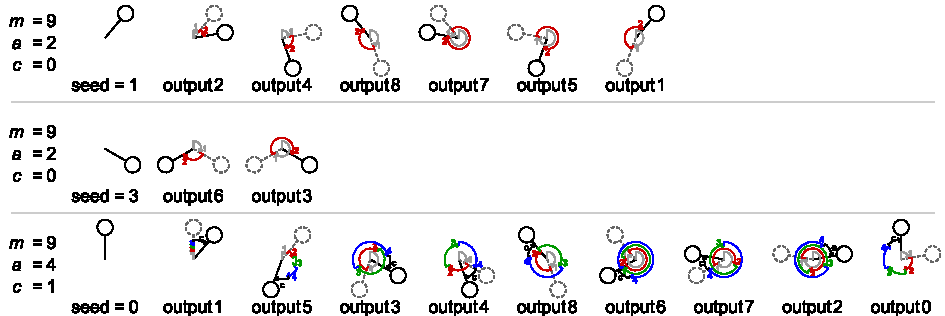
\includegraphics[width=0.8\textwidth]{figures/lcg.pdf}
    \caption{The cycle length of a linear congruential generator depends on the parameters and seed.}
    \label{fig:lcg}
\end{figure}

Examples of LCGs are ANSI-C, RAND, drand48 and NAG (NAG with period of $2^{48}$).

\redbox{While LCGs are fast and require minimum storage, but they show regular patterns. For instance if
you generate lots of random numbers and from them take bunches of $k$ and plot them in a $k$-dimensional space, you will see
they lie on at most $(k! \cdot m)^{1\slash k}$ parallel $k-1$-dimensional hyperplanes. Also, if $m$ is chosen as a power of $2$ (as in the
subsequently discussed RANDU), the least significant bits are not very random (the least significant one has a period
of at most $2$).}

Let us present RANDU, an infamous, simple linear congruential generator (LCG), given by
\begin{equation}
    v_{n+1} = (65539 \cdot v_n) \mod 2^{31}, \quad \text{seed } v_0, \quad \text{pseudo-random number } u_n = \frac{v_n}{2^{31}}
\end{equation}
where based on an integer sequence uniformly distributed numbers $u_n$ are generated. Now RANDU is not infamous because it is especially good, but rather
because it is especially bad in the sense that generated numbers are closely related, as illustrated in figure \ref{fig:randu}.

\begin{figure}[H]
    \centering
    \includesvg[width=0.8\textwidth]{figures/randu.svg}
    \caption{Consecutive numbers generated by RANDU plotted in 2D lie on parallel lines.}
    \label{fig:randu}
\end{figure}

A more in-depth discussion about the problems of RANDU and linear congruential
generators in general can be found in \cite[chapter 7]{press07}, where more advanced 
methods are also discussed. In R for instance the default number generator is the 
Marsenne-Twister \citep{matsumoto98} according to the 
\href{https://cran.r-project.org/web/views/Distributions.html}{Comprehensive R Archive Network}.

\subsubsubsection{A first improvement | Combining multiple LCGs}
\begin{equation}
    \left.\begin{array}{rl}
    X_{i+1} & =\left(40014 X_i\right) \bmod 2147483563 \\
    Y_{i+1} & =\left(40692 Y_i\right) \bmod 2147483399 \\
    Z_{i+1} & =\left(X_i+Y_i\right) \bmod 2147483563
    \end{array}\right\} \rightarrow \text { then map } Z_i \text { to floating point number }
\end{equation}

\subsubsubsection{Lagged Fibonacci Generators}
Inspired by the Fibonacci series, we combine \textit{lagged numbers}, i.e. numbers
earlier in the series by offsets $p$ and $q$

\begin{equation}
    v_i = (v_{i-p} \odot v_{i-q}) \mod m
\end{equation}

where $\odot$ is some arithmetic operation like addition or bitwise XOR.
For instance the Mersenne Twister is based on such
a method and has period $2^{19937} - 1$.

\subsubsubsection{Roughly evenly spaced sampling - blue noise}
Randomly sampled points in 2D will not be evenly spread - 
if we want more even sampling, \textit{blue noise}
generated for instance by Fast Poisson Disk sampling 
(sampled points are at least $r$ apart, $\mathcal{O}(N)$, $N$ sampled points) can be used.

Blue noise and usual randomly sampled numbers 
are shown in table \ref{tab:bluenoise}. For 
instance the photoreceptors on our retina are
laid out in a blue noise fashion.

\begin{table}[H]
    \centering
    \begin{tabular}{c|c}
        \textcolor{blue1}{Random numbers using math.random()} & \textcolor{blue1}{Blue noise using Poisson Disk Sampling} \\
        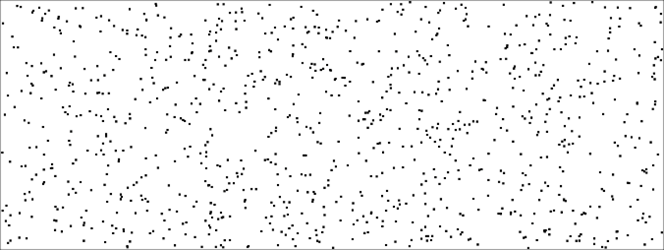
\includegraphics[width=0.4\textwidth]{figures/random.png} & 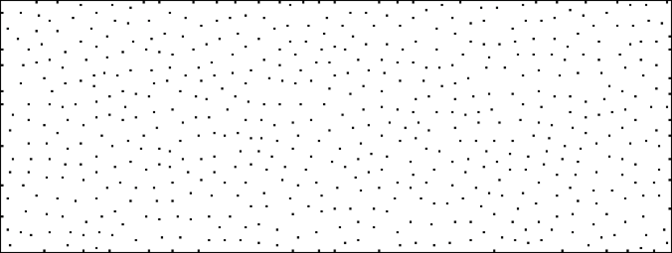
\includegraphics[width=0.4\textwidth]{figures/bluenoise.png}
    \end{tabular}
    \caption{Randomly sampled points in 2D (left) and blue noise (right).}
    \label{tab:bluenoise}
\end{table}

\subsubsection{Inverse Transform Method | sampling from distributions with algebraically invertible cumulative distribution functions (CDFs)}
Consider we want to sample from a distribution with PDF $f(x)$ and
cumulative distribution function (CDF) $F(x) = \int_{-\infty}^x f(x') dx'$. Given a uniformly distributed variable
$U \sim \mathcal{U}(0,1)$, $F^{-1}(U)$ is distributed according to $f$, as
\begin{equation}
    P(F^{-1}(U) \leq x) = P(U \leq F(x)) = F(x), \quad x \in \mathbb{R}
\end{equation}
where we used that as of $f(x) \geq 0$, $F(x)$ is monotonically increasing, so its application keeps the inequality intact.

This is the foundation of the inverse transform method which is implemented in R in code-snippet \ref{code:inverse_transform} and illustrated
at the hand of sampling from a Gaussian in figure \ref{fig:gaussian_inverse}. Note that the inverse transform method would actually not
be used on a Gaussian as the inverse of its CDF has no closed-form expression and e.g. the Box-Muller method \citep{box58}
would be used.

\begin{codebox}[!htb]
    \begin{minted}{R}
        inverse_transform_method <- function(n, F_inv) {
            # Draw n samples from a distribution with CDF F
            # given its inverse F_inv.
            u <- runif(n) # draw n samples from U(0,1)
            return(F_inv(u)) # apply the inverse transform
        }
    \end{minted}
    \caption{Inverse Transform Method in R}
    \label{code:inverse_transform}
\end{codebox}

\begin{figure}[!htb]
 \centering
 \includesvg[width=1.0\textwidth]{figures/exact_inversion.svg}\hfill
 \caption{Illustration of the Inverse Transform Method}
 \label{fig:gaussian_inverse}
\end{figure}

\problem{Not all CDFs are algebraically invertible.}
\idea{Numerical inversion is just swapping the axes - but we have discrete inverted point with 
different spacing. One idea is to linearly interpolate in the to find $F^{-1}$ at the uniformly distributed points.}

\subsubsubsection{Alternative derivation from the transformation between probability distributions\skipthis}
Consider probability distributions $f_1(x), f_2(y)$ with $y = y(x)$. Conservation of total probability implies
\begin{equation}
    f_1(x) dx = f_2(y) dy \quad \rightarrow \quad f_2(y) = f_1(x) \left| \frac{dx}{dy} \right|
\end{equation}
so the cumulative distribution functions are equal (?)
\begin{equation}
    F_1(x)=\int_{-\infty}^x F_1(\tilde{x}) d \tilde{x}=\int_{-\infty}^y f_2(\tilde{y}) d \tilde{y}=F_2(y(x))
\end{equation}
so taking $f_1(x)$ as the uniform distribution, $F_1(x) = x$ and we get to the same result.

\subsubsubsection{Example: Inverse Transform Method applied to the standard Laplace distribution\skipthis}

The standard Laplace distribution is given by the PDF
\begin{equation}
    f(x) = \frac{1}{2} e^{-|x|}, \quad x \in \mathbb{R}
\end{equation}
with the CDF following from $F(x) = \int_{-\infty}^x f(x') dx'$ to
\begin{equation}
    F(x) = \begin{cases}
        \frac{1}{2} e^x & \text{if } x \leq 0 \\
        1 - \frac{1}{2} e^{-x} & \text{if } x > 0
    \end{cases}
\end{equation}
with the inverse CDF
\begin{equation}
    F^{-1}(u) = \begin{cases}
        \ln(2u) & \text{if } u \leq \frac{1}{2} \\
        -\ln(2(1-u)) & \text{if } u > \frac{1}{2}
    \end{cases}
\end{equation}
where $\frac{1}{2}$ as the transitioning point between the pieces follows intuitively from the symmetry of the PDF around $x=0$.

The results are illustrated in figure \ref{fig:laplace_inverse}.

\begin{figure}[!htb]
 \centering
 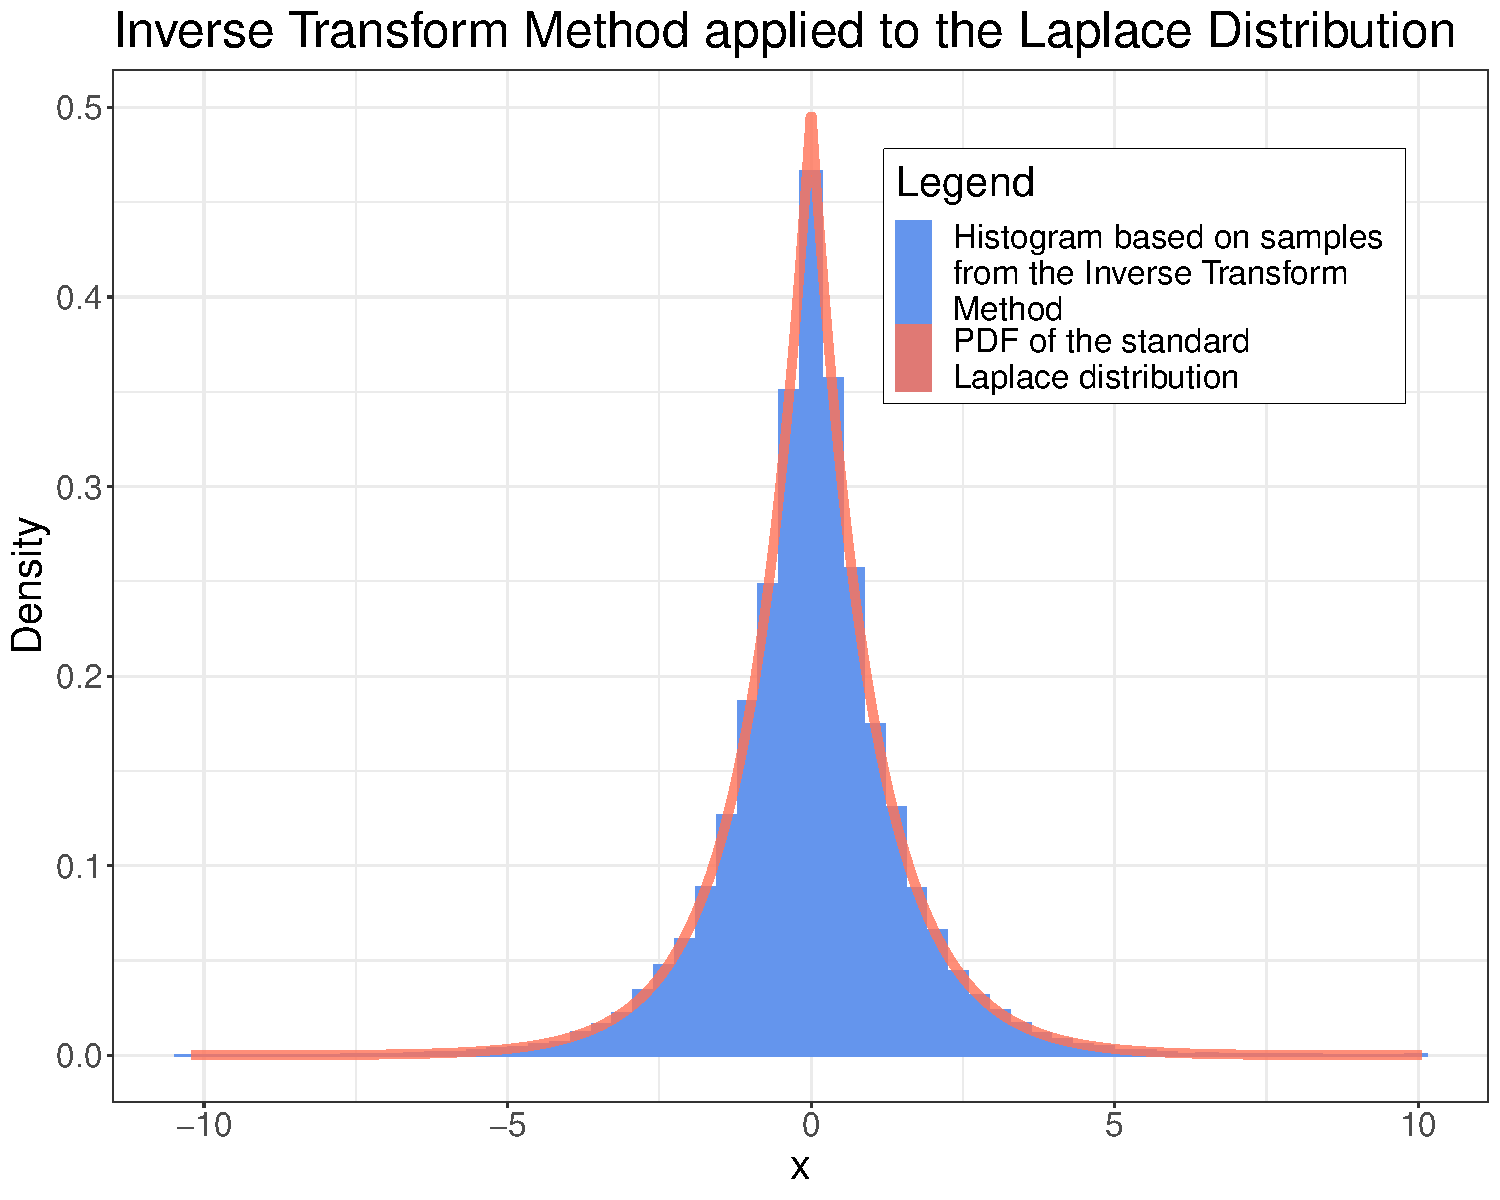
\includegraphics[width=1.0\textwidth]{figures/laplace_inverse.pdf}\hfill
 \caption{Illustration of the Inverse Transform Method applied to the standard Laplace distribution}
 \label{fig:laplace_inverse}
\end{figure}

\subsubsubsection{Sampling from a Gaussian using exact inversion | Box-Muller trick}
We want to sample from the Gaussian
\begin{equation}
    f(y) = \frac{1}{\sqrt{2\pi}} \exp{\left(-\frac{y^2}{2}\right)}
\end{equation}
\problem{The CDF is the error function, which has no closed-form inverse.}
\idea{In the Box-Muller trick, a 2D Gaussian in polar coordinates is inverted.}

Consider the 2D Gaussian

\begin{equation}
    f(x, y)=\frac{1}{2 \pi} \exp \left(-\frac{x^2+y^2}{2}\right)
\end{equation}

note that we can also write this in polar coordinates $x = r \cos(\theta), y = r \sin(\theta)$ ($r^2 = x^2 + y^2$) as
the product of an independent radial and angular probability distribution

\begin{equation}
    f(x, y) \, dx \, dy = \mathcolor{green1}{f(\phi)} \, d\phi \cdot \mathcolor{blue1}{f(r)} \, dr = \mathcolor{green1}{\frac{1}{2 \pi}} \mathcolor{blue1}{\exp \left(-\frac{r^2}{2}\right) r} \, dr \, d\phi
\end{equation}

where based on random numbers $u_1, u_2 \sim \mathcal{U}(0,1)$ we can sample both $r$ and $\phi$ by exact inversion.

\begin{equation}
    \begin{aligned}
        u_1 & = \frac{1}{2\pi} \phi \quad \rightarrow \quad &\phi = 2\pi u_1 \\
        u_2 & = \int_{0}^{r} \exp \left(-\frac{r'^2}{2}\right) \, dr'= 1 - \exp \left(-\frac{r^2}{2}\right) \quad \rightarrow \quad & r = \sqrt{-2 \ln(1 - u_2)}
    \end{aligned}
\end{equation}

As the 2D Gaussian is just a product of 1D Gaussians, from $r$ and $\phi$ we can then get two normally distributed numbers $x$ and $y$.

\bluebox{\textbf{Box-Buller trick:} Given two uniformly distributed random numbers $u_1, u_2 \sim \mathcal{U}(0,1)$, we can generate two normally distributed random numbers $x, y \sim \mathcal{N}(0,1)$ by
\begin{equation}
    \phi = 2\pi u_1, \quad r = \sqrt{-2 \ln(1 - u_2)} \quad \rightarrow \quad x = r \cos(\phi), \quad y = r \sin(\phi)
\end{equation}
}

\subsubsubsection{Sampling from a discrete distribution\skipthis}

Consider a random variable $X$ with the following probability mass function

\begin{equation}
    P(X = x) = \begin{cases}
        0.1 & \text{if } x = 0 \\
        0.15 & \text{if } x = 1 \\
        0.25 & \text{if } x = 2 \\
        0.3 & \text{if } x = 3 \\
        0.2 & \text{if } x = 4 \\
        0 & \text{otherwise}
    \end{cases}
    \label{eq:discrete}
\end{equation}

Intuitively sampling according to such a discrete distribution is simple: 
For uniform draws between $0$ and $1$, each section $a \le x < b$ within has a probability $b - a$.
Therefore, we only have to associate each $x$ with a section of length $P(X = x)$.

The sections we are interested in are directly given by the cumulative distribution function, as illustrated in
figure \ref{fig:discrete_transform}.

\begin{figure}[!htb]
 \centering
 \includesvg[width=1.0\textwidth]{figures/discrete_inverse_transform.svg}\hfill
 \caption{Illustration of the Inverse Transform Method applied to the standard Laplace distribution}
 \label{fig:discrete_transform}
\end{figure}

\subsubsection{Acceptance-rejection method}
Let's say we want to sample from a complex distribution $p(x)$ and we can sample from a simple distribution $f(x)$ with
$p(x) \leq C f(x)$, some constant $C$.

We can then draw samples from $p(x)$ using the Acceptance-Rejection method, consisting of the following steps:
\begin{enumerate}
    \item Generate a trial value $x$ from $f(x)$ (e. g. using exact inversion)
    \item Generate a value $y$ from a uniform distribution $0\leq y<C f(x)$
    \item If $y\leq p(x)$ return $x$ as the sample value
    \item Else, reject the trial value $x$ and draw again
\end{enumerate}

An illustration is provided in figure \ref{fig:acceptance_rejection}.

\begin{figure}[!htb]
 \centering
 \includesvg[width=1.0\textwidth]{figures/acc_rej.svg}\hfill
 \caption{Illustration of the Acceptance-Rejection Method}
 \label{fig:acceptance_rejection}
\end{figure}
 
\textbf{Intuition}: The logic behind this is very clear if we just choose $f(x)=const$. i. e. we uniformly sample $x$. This, however, would be very inefficient, so we use $ C f(x)$ that lies on top $p(x)$ as closely as possible.
\par
\textbf{Proof that we get the correct distribution:} The probability $dq$ to get (accept) a certain $x$ within $dx$ is

\begin{equation}
    dq = \explain{f(x) dx}{from step 1} \explain{\frac{p(x)}{C f(x)}}{step 2 to 4} = \frac{1}{C} p(x) dx \propto p(x) dx
\end{equation}

\greenbox{\textbf{Advantages}:\begin{itemize}
    \item works in any dimension
    \item $p(\vec{x})$ does not have to be normalized (in contrast to exact inversion)
\end{itemize}}
\redbox{\textbf{Disadvantages}: Note that this is very inefficient if the rejection area is large and efficiency rapidly decreases in higher dimensions (then one might try to construct samples through a stochastic process).}

\subsubsubsection{Example: Sampling uniformly from a sphere}
\bluebox{\textbf{Aim: } Uniformly sample points from the surface of a sphere.}
In 3D we can use exact inversion to sample from the surface. The surface element in spherical coordinates is
\begin{equation}
    dS = r^2 \sin(\theta) \, d\theta \, d\phi = r^2 \, d cos(\theta) \, d\phi
\end{equation}
(sign?) so $d cos(\theta) d\phi$ and $d \phi$ are uniform over their range. So we can use
\begin{equation}
    \cos \theta = 1 - 2u_1, \quad \phi = 2\pi u_2, \quad u_1, u_2 \sim \mathcal{U}(0,1)
\end{equation}
so we can sample from the surface of a sphere by
\begin{equation}
    \begin{aligned}
        x &= r \sin(\theta) \cos(\phi) \\
        y &= r \sin(\theta) \sin(\phi) \\
        z &= r \cos(\theta)
    \end{aligned}
\end{equation}

\problem{Generalization to higher dimensions is not straightforward.}

\idea{Use the acceptence-rejection method.}
\begin{itemize}
    \item Uniformly sample $u_1, u_2, u_3 \sim \mathcal{U}(0,1)$
    \item If $r_d = u_1^2 + u_2^2 + u_3^2 \leq 1$, return $(u_1, u_2, u_3)$, else reject and draw again
    \item Project the points to the surface of the unit sphere by
    \begin{equation}
        \begin{aligned}
            x &= \frac{u_1}{r}
            y &= \frac{u_2}{r}
            z &= \frac{u_3}{r}
        \end{aligned}
    \end{equation}
\end{itemize}
which can easily be extended to higher dimensions.

\subsubsubsection{Example II: Sampling from a conditioned Gamma distribution\skipthis}

We would like to sample from $Gamma(2,1)$ conditional on the random variable being greater than $5$, i.e.
\begin{equation}
    p(x) = \begin{cases}
        \frac{x \exp(-x)}{6\exp(-5)} & \text{if } x \geq 5 \\
        0 & \text{otherwise}
    \end{cases}
\end{equation}
(normalized). We use the acceptance-rejection method with $f(x)$ being an exponential distribution with $\lambda = 0.5$ conditional on the random variable being greater than $5$, i.e.
\begin{equation}
    f(x) = \begin{cases}
        \frac{1}{2 \exp\left(-\frac{5}{2}\right)} \exp(-\frac{x}{2}) & \text{if } x \geq 5 \\
        0 & \text{otherwise}
    \end{cases}
\end{equation}

which we have normalized. We can draw from $f(x)$ using the inverse transform method, where we can e.g. efficiently take care of the conditioning by
drawing uniformly between $\int_{0}^{5} \frac{1}{2} \exp(-\frac{x}{2}) dx = 1 - \exp\left(-\frac{5}{2}\right)$ and $1$ in the inverse transform method.

The result is illustrated in figure \ref{fig:exp_conditional}.

\begin{figure}[!htb]
    \centering
    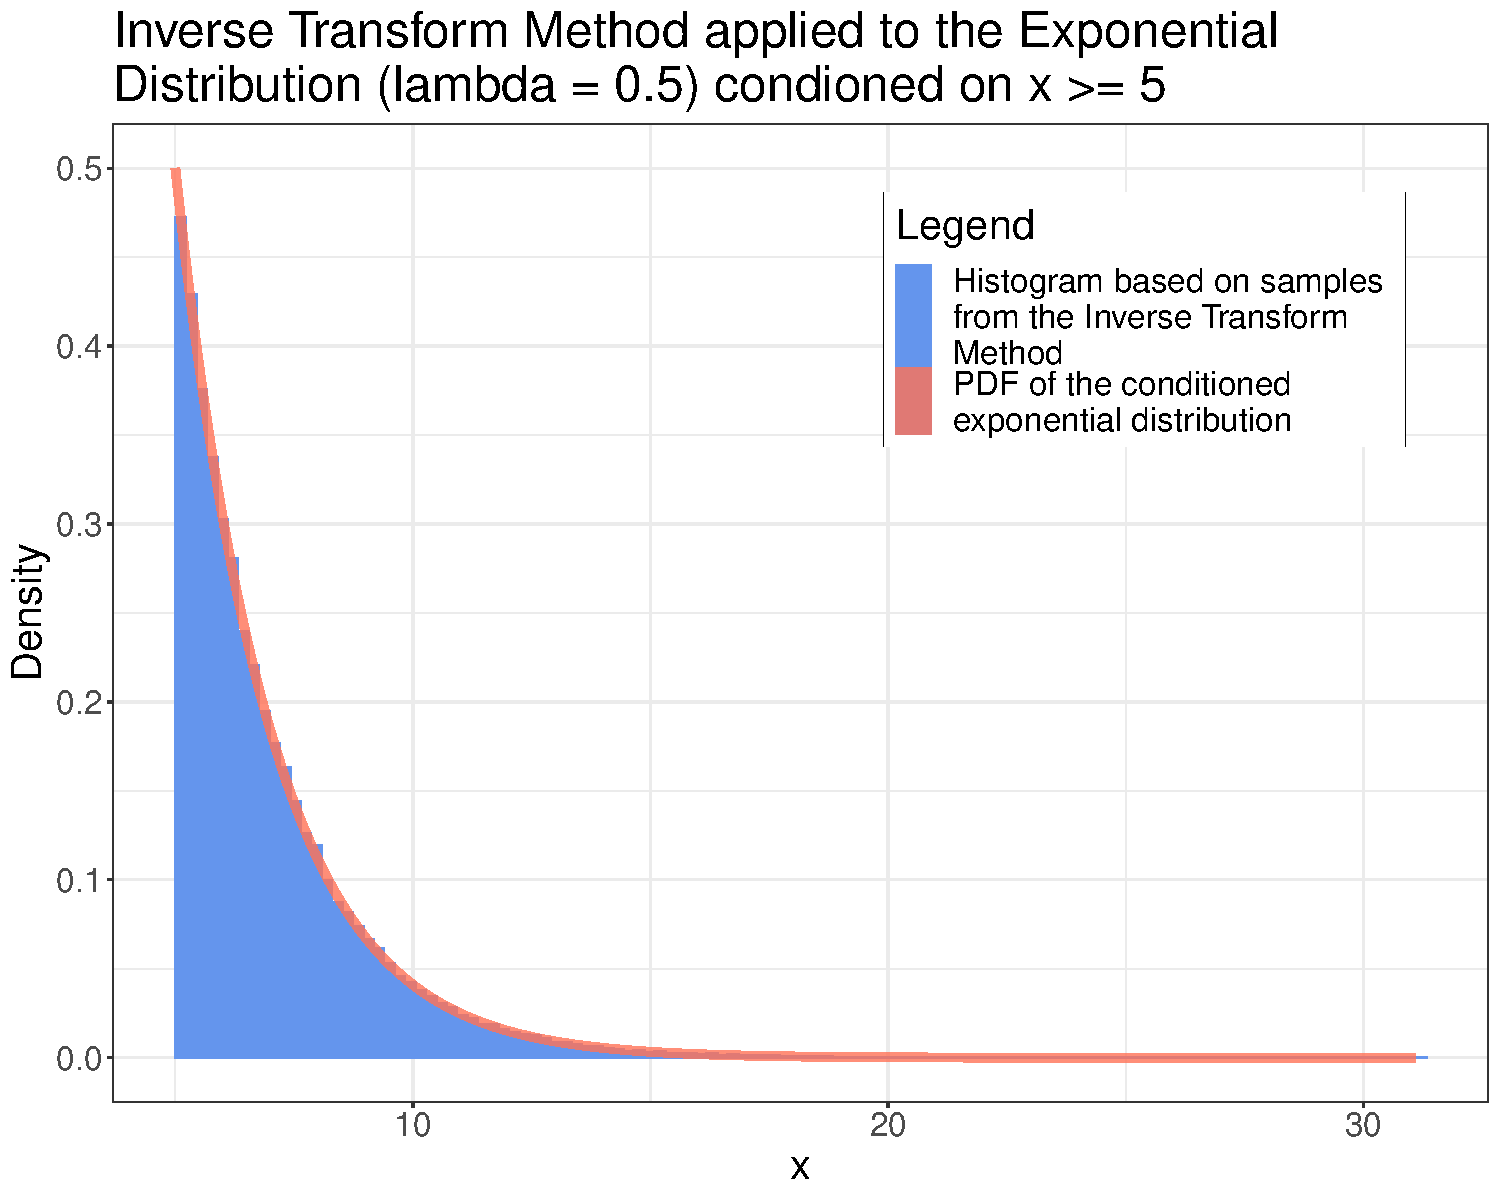
\includegraphics[width=1.0\textwidth]{figures/exp_conditional.pdf}\hfill
    \caption{Application of the Inverse Transform Method to sample from a conditioned Exponential distribution}
    \label{fig:exp_conditional}
\end{figure}

As for both the exponential and the gamma distribution of consideration for $x\geq 5$ the PDFs are monotonically decreasing, for $C$ in the acceptance-rejection method, we can use
\begin{equation} {
    C = \frac{p(5)}{f(5)} = \frac{5}{3}
}
\end{equation}

The results from applying the acceptance-rejection method are illustrated in figure \ref{fig:gamma_conditional}.

\begin{figure}[!htb]
    \centering
    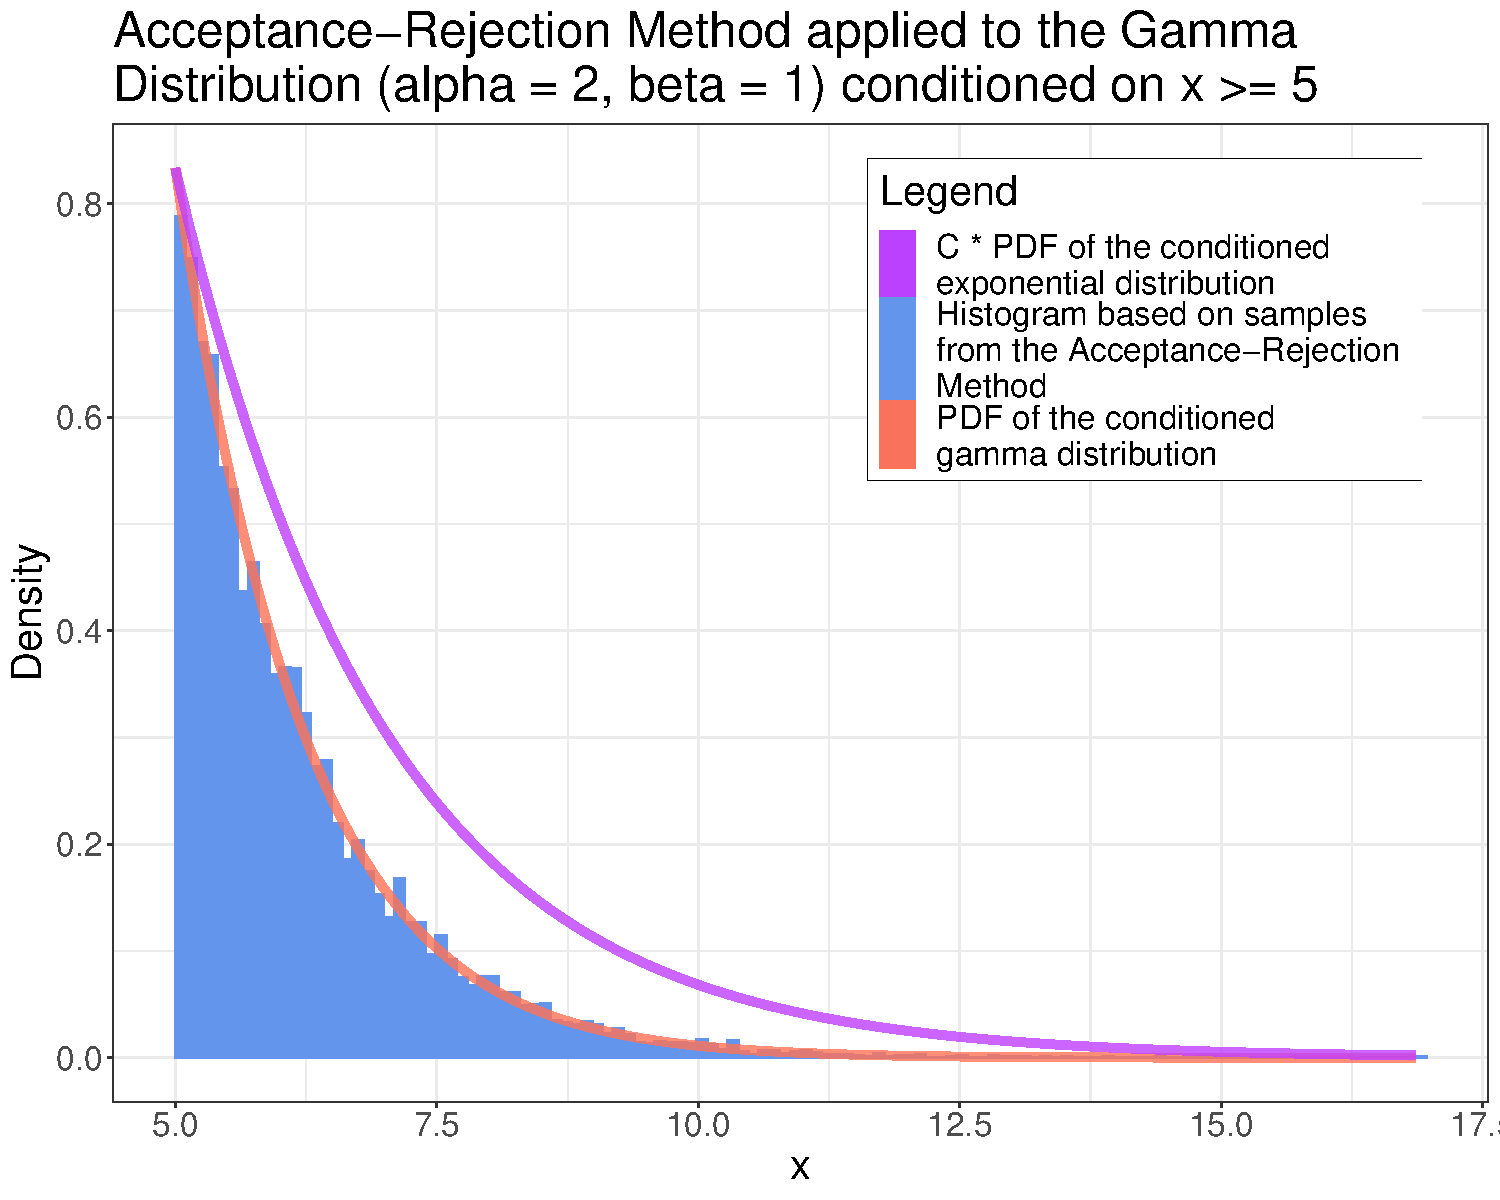
\includegraphics[width=1.0\textwidth]{figures/gamma_conditional.pdf}\hfill
    \caption{Application of the Acceptance-Rejection Method to sample from a conditioned Gamma distribution}
    \label{fig:gamma_conditional}
\end{figure}

\subsection{Monte Carlo Estimation}

\subsubsection{A basic intuition for estimation}
We generally draw information about reality from samples. Consider for instance we measure the energy deposited
by energetic muons in a thin silicon layer. We might measure (for different muons of the same energy) 
$X = [0.5 \MeV, 0.6 \MeV, 1.3 \MeV]$ and we might say that in the mean the energy deposit might in general be $0.8 \MeV$ (without
knowing the true distribution, from which we sampled; here quite intricate, see \cite[figure 34.7]{particle2020}).
\par
We have just declared our sample estimator to be at least an approximation for the population parameter - which
might not be a good idea, especially for such a small sample size.

\subsubsection{Monte Carlo Estimation}
Monte Carlo Estimation is concerned with estimating statistics by approximating their expectations. So for a random variable with
probability distribution $f(x)$ (continuous or discrete) the expectation of a function $g$, so

\begin{equation}
    \theta := E[g(X)] = \begin{cases}
        \sum_{k=1}^{\infty} g(x_k) \cdot f(x_k) & \text{if } X \text{ is discrete} \\
        \int_{-\infty}^{\infty} g(x) \cdot f(x) dx & \text{if } X \text{ is continuous}
    \end{cases}
\label{eq:mc_est}
\end{equation}

is approximated by a sample mean over $(X_1, \dots, X_m)$ ($m$ independent realizations from the distribution of $X$)

\begin{equation}
    \hat{\theta} := \frac{1}{m} \sum_{i=1}^{m} g(X_i)
\end{equation}

which is an unbiased estimator for $\theta$ if the expectation exists and converges almost surely to $\theta$ in the limit of a large sample size (by the strong law of large numbers).

\subsubsection{Distribution and Error of the Monte Carlo Estimator}
Assume that $\Var[g(X)] = \sigma^2 < \infty$. Then by the basic properties of the variance, we can write

\begin{equation}
    \Var[\hat{\theta}_m] = \frac{1}{m^2} \sum_{i=1}^{m} \Var[g(X_i)] = \frac{\sigma^2}{m}
\end{equation}

Notice that for the distribution of our sample mean (an addition of $m$ i.i.d random variables) the central limit theorem applies, so

\begin{equation}
    \frac{\hat{\theta}_m - \theta}{\sigma / \sqrt{m}} \xrightarrow[m \rightarrow \infty]{d} Z \sim \mathcal{N}(0, 1)
\end{equation}

We would like to use the above to specify confidence intervals for our estimator $\hat{\theta}_m$. Note, however,
that $\sigma$ is unknown to us. Luckily, the above still holds in the limit of a large sample size when using the
estimator

\begin{equation}
    S_n^2 := \frac{1}{m-1} \sum_{i=1}^{m} (g(X_i) - \hat{\theta}_m)^2
\end{equation}

or rather the square root $S_n$. Notice that while $S_n$ is, different from $S_n^2$, not an unbiased estimator, it converges
in probability to $\sigma$ which is sufficient to apply Slutsky's theorem yielding

\begin{equation}
    \frac{\hat{\theta}_m - \theta}{S_n / \sqrt{m}} \xrightarrow[m \rightarrow \infty]{d} Z \sim \mathcal{N}(0, 1)
\end{equation}

\subsection{Monte Carlo Integration}
Classical numerical methods for integration (e.g. Simpson's rule) become infeasible for high-dimensional integrals,
essentially, as the errors scale with the number of function-evaluation-points per dimension (so in high dimensions, we need
to perform lots of function evaluations).

\subsubsection{Intuition for Monte Carlo Integration}
Consider we want to calculate the integral

\begin{equation}
    I := \int_{V} g(\vec{x}) d^d \vec{x}
\end{equation}

where $V$ is a $d$-dimensional volume and $g$ is a function $g: V \rightarrow \mathbb{R}$. Then it makes intuitive sense
to approximate this integral by the mean of the function $g$ on the domain of interest, as found as the mean of $g$ evaluated
at $N$ random points $\vec{x}_i$ in $V$, multiplied by the volume of $V$ (also denoted by $V$)

\begin{equation}
\hat{I}_N := \frac{V}{N} \sum_{i=1}^{N} g(\vec{x}_i) \xrightarrow[N \rightarrow \infty]{a.s.} I
\end{equation}

\bluebox{\textbf{Monte Carlo Integration}: Let $V$ for simplicity be the hypercube $[0,1]^d$ (by change of variables, the domain of interest can be mapped to this hypercube). Then Monte Carlo
integration to approximate $I = \int_{[0,1]^d} g(\vec{x}) d^d \vec{x}, \vec{x} \in \mathbb{R}^d$ is given by
\begin{itemize}
    \item Generate $N$ random vectors $\vec{x}$ where each component is drawn uniformly from $[0,1]$ (so we need $N\times d$ random numbers)
    \item Evaluate
    \begin{equation}
        \hat{I}_N = V \frac{1}{N} \sum_{i=1}^{N} g(\vec{x}_i), \quad \text{here } V = 1 
    \end{equation}
\end{itemize}}

\greenbox{\textbf{Scaling of the error}: The error of the Monte Carlo integrator scales with $1/\sqrt{N}$, independent of the number of dimensions of the integration $d$.}

\subsubsection{Connection to the Monte Carlo Estimator}
We can also obtain the result from above
from the Monte Carlo Estimator (eq. \ref{eq:mc_est}) by using the uniform distribution
\begin{equation}
    f(\vec{x}) = \begin{cases}
        \frac{1}{V} & \text{if } \vec{x} \in V \\
        0 & \text{else}
    \end{cases}
\end{equation}
and rewriting the integral as
\begin{equation}
    I = \int_{V} g(\vec{x}) d^d \vec{x} = V \int_{V} g(\vec{x}) \cdot \frac{1}{V} d^d \vec{x} = V \int_{V} g(\vec{x}) \cdot f(\vec{x}) d^d \vec{x}
\end{equation}

\subsubsection{Intuition from calculating the area of a shape}
Consider an irregular shape with area $A_{\text{shape}}$ within a rectangle with area $A_{\text{rect}}$. 
The probability that a point drawn uniformly from the rectangle lies within the shape is 
\begin{equation}
    p_{\text{shape}} = \frac{A_{\text{shape}}}{A_{\text{rect}}}
\end{equation}
so we can approximate
\begin{equation}
    A_{\text{shape}}\approxeq A_{\text{rect}} \frac{\# \text{ hits in shape}}{\# \text{ hits in rectangle}}
\end{equation}
which is the same as the Monte Carlo Integration introduced, where $g(\vec{x}) = 1_{\text{shape}}(\vec{x})$ and $V = A_{\text{rect}}$.

\subsubsection{Error in Monte Carlo Integration - scaling with $\frac{1}{\sqrt{N}}$}
Based on the connection to the Monte Carlo Estimator, the
variance of our estimator for the integral is given by
\begin{equation}
    \Var[\hat{I}_N] = \frac{V^2}{N} \Var[g(x)], \quad \text{estimate} \Var[g(x)] \text{ by } S_{g;N}^2 := \frac{1}{N-1} \sum_{i=1}^{N} \left(g(x_i) - \frac{\hat{I}_N}{V}\right)^2
    \label{eq:mcint_var}
\end{equation}
\bluebox{
So the standard error of our Monte Carlo estimator
\begin{equation}
    \hat{I}_N = \frac{V}{N} \sum_{i=1}^{N} g(\vec{x}_i)
\end{equation}
that is if we calculate $\hat{I}_N$ multiple times with different random samples, the standard deviation of these
different estimates is
 \begin{equation}
    \boxed{\sigma_{\hat{I}_N} = V \sqrt{\frac{\sigma_g^2}{N}} \propto \frac{1}{\sqrt{N}}}
 \end{equation}
which is illustrated in figure \ref{fig:mcint}. This follows directly from the basic properties of the variance
\begin{equation}
    \text{for } X,Y \text{ independent} \quad \Var[X+Y] = \Var[X] + \Var[Y], \quad \Var[aX] = a^2 \Var[X]
\end{equation}
with
\begin{equation}
    \Var[\hat{I}_N] = \Var\left[\frac{V}{N} \sum_{i=1}^{N} g(\vec{x}_i)\right] = \frac{V^2}{N^2} \sum_{i=1}^{N} \Var[g(\vec{x}_i)] \underset{\vec{x}_i \text{ i.i.d.}}{=} \frac{V^2}{N} \Var[g(\vec{x})]
\end{equation}
}

\subsubsection{Distribution of $\hat{I}_N$ and derivation of the central limit theorem\skipthis}
The Monte Carlo Estimator is
\begin{equation}
    \hat{I}_N = \frac{V}{N} \sum_{i=1}^{N} g(\vec{x}_i) = \frac{1}{N} \sum_{i=1}^{N} y_i = \sum_{i=1}^{N} s_i, \quad y_i = V g(\vec{x}_i), \quad s_i = \frac{y_i}{N}
\end{equation}
by basic properties of variance and mean
\begin{equation}
    \begin{gathered}
        \langle \hat{I}_N \rangle = N \langle s \rangle = \langle y \rangle  \\
        \Var[\hat{I}_N] = N \Var[s] = \frac{1}{N} \Var[y] = \frac{V^2}{N} \Var[g(\vec{x})]
    \end{gathered}
\end{equation}
\note{$p(y)$ is the distribution of $y$ over $V$ along the $y$-axis with
\begin{equation}
    \langle y \rangle = \int y p(y) \, dy = \int_{V} g(\vec{x}) \, d^d \vec{x}, \quad \int p(y) \, dy = 1
\end{equation}
\textbf{$p(y)$ might be any distribution.}
}
Applying the Central Limit Theorem (eq. \ref{eq:central_limit_theorem}) to the Monte Carlo Estimator
(assuming the moments of $p(y)$ exist and are finite), we obtain
\begin{equation}
    \begin{aligned}
        P_N(\hat{I}_N) &= \frac{1}{\sqrt{2\pi \Var[\hat{I}_N]}} \exp{\left( -\frac{(\hat{I}_N-\langle \hat{I}_N \rangle)^2}{2\Var[\hat{I}_N]} \right)} \\
                       &= \frac{\sqrt{N}}{\sqrt{2\pi \sigma_y^2}} \exp{\left( -\frac{N(\hat{I}_N-\langle y \rangle)^2}{2\sigma_y^2} \right)}
    \end{aligned}
\end{equation}
independent of the shape of $p(y)$ for $N$ sufficiently large.

\paragraph{Derivation of the Central Limit Theorem by Fourier Transform} The central limit
theorem can be derived by considering $P_N$ in Fourier space, where 
the central ingredient will simply be
\begin{equation}
    \exp{x} = \lim_{N \rightarrow \infty} \left(1 + \frac{x}{N}\right)^N
\end{equation}
which is also approximately true for large $N$.
\bluebox{\textbf{Distribution of the sum of independent random variables}: Consider \textbf{independent} variables $X,Y$ with PDFs $f_X$ and $f_Y$. The PDF of the sum $Z = X + Y$
is naturally the convolution
\begin{equation}
    f_Z(z)=\int_{-\infty}^{\infty} \underbrace{f_X(x) f_Y(z-x)}_{x+(z-x) = z} d x
\end{equation}
Another way to write this is
\begin{equation}
    f_Z(z)=\int f_X(x) f_Y(y) \delta(z-(x+y)) \, d x \, d y
\end{equation}
which one can easily see is equivalent to the convolution and also makes intuitive sense - the $\delta$-function
ensures that the sum of $x$ and $y$ is $z$.
}
Analogously to the two-variable case, we write
\begin{equation}
    P_N\left(\hat{I}_N\right)=\int \delta\left(\hat{I}_N-\sum_i \frac{y_i}{N}\right) p\left(y_1\right) p\left(y_2\right) \cdots p\left(y_N\right) \mathrm{d} y_1 \mathrm{~d} y_1 \cdots \mathrm{d} y_N
\end{equation}
Based on the Fourier transform and expansion of $p(y)$
\begin{equation}
    \begin{aligned}
        \hat{p}(k)&=\int p(y) \exp{\left(i k(y-\langle y\rangle)\right)} \, \mathrm{d} y \\
        \underset{\text{Series Expansion}}&= \int p(y) \left[ 1 + ik(y-\langle y\rangle) - \frac{k^2}{2}(y-\langle y\rangle)^2 + \cdots \right] \, \mathrm{d} y \\
        &= 1 - \frac{k^2}{2} \sigma_y^2 + \cdots
    \end{aligned}
\end{equation}
we find the Fourier transform of $P_N$ to be
\begin{equation}
    \begin{aligned}
    \hat{P}_N(k) & =\int P_N\left(\hat{I}_N\right) \exp{\left(i k\left(I_N-\left\langle I_N\right\rangle\right)\right)} \mathrm{d} I_N \\
    \underset{\langle \hat{I}_N \rangle = \langle y \rangle}&= \int p\left(y_1\right) \cdots p\left(y_N\right) \exp{\left(i \frac{k}{N}\left(y_1-\left\langle y_1\right\rangle+y_2-\left\langle y_2\right\rangle+\ldots+y_N-\left\langle y_N\right\rangle\right)\right)} \mathrm{d} y_1 \cdots \mathrm{d} y_N \\
    &= \left[\hat{p}\left(\frac{k}{N}\right)\right]^N \\
    \underset{\text{series expansion of } \hat{p}}&= \left( 1 - \frac{k^2 \sigma_y^2}{2N^2} \right)^N \\
    \underset{N \text{ large}}&\approxeq \exp{\left( - \frac{k^2 \sigma_y^2}{2N} \right)}
    \end{aligned}
\end{equation}
where the inverse Fourier transform of $\hat{P}_N(k)$
\begin{equation}
    P_N\left(\hat{I}_N\right)=\frac{1}{2 \pi} \int \exp{\left(-i k\left(I_N-\left\langle I_N\right\rangle\right)\right)} \hat{P}_N(k) \mathrm{d} k
\end{equation}
yields the previously stated result for $P_N\left(\hat{I}_N\right)$\footnote{Insert the result for $\hat{P}_N(k)$, complete the square and use the normalization of the normal distribution
or the Gaussian integral $\int \exp \left(-\alpha x^2\right) \mathrm{d} x=\sqrt{\frac{\pi}{\alpha}}$.}.

\subsubsection{Illustrative Example of Monte Carlo Integration}
Consider the integral
\begin{equation}
    I = \int_{0}^{1} g(x) dx, \quad g(x) = \exp{\left(-\frac{x^2}{2}\right)}
\end{equation}
Our Monte Carlo estimator for this integral is given by
\begin{equation}
    \hat{I}_N = \frac{1}{N} \sum_{i=1}^{N} g(x_i), \quad x_i \sim \mathcal{U}(0, 1)
\end{equation}
which is illustrated in figure \ref{fig:mcint}. The higher the number of sampled points $N$ the lower the variance of our estimator; the lower the variance of $g$ along the $y$ axis, the lower the variance of our estimator.

\begin{figure}[!htb]
 \centering
 \includesvg[width=1\textwidth]{figures/mc_int.svg}\hfill
 \caption{Illustration of Monte Carlo Integration for $I = \int_{0}^{1} \exp{\left(-\frac{x^2}{2}\right)} dx$}
 \label{fig:mcint}
\end{figure}

\subsubsection{Comparison to other techniques - when to use Monte Carlo integration?}
\paragraph*{Error of standard methods} In a standard integration scheme like the midpoint rule
or Simpsons rule\footnote{$\int_a^b f(x) d x \approx \frac{b-a}{6}\left[f(a)+4 f\left(\frac{a+b}{2}\right)+f(b)\right]$
which can be derived by approximating the function $f$ by a quadratic polynomial and integrating this polynomial.} each
dimension is divided into $n$ regularly space points, so that we have $N = n^d$ points in total. The error scales with
\begin{equation}
    \text{midpoint or trapezoidal rule } \propto \frac{1}{n^2}, \quad \text{Simpson's rule } \propto \frac{1}{n^4} = \frac{1}{N^{\frac{4}{d}}}
\end{equation}
\redbox{In these \textit{regular} methods, adding more points to the integration (increasing $N$) helps less and less the higher we go 
in dimension - e.g. for Simpson's rule $\text{err} \propto \frac{1}{N^{\frac{4}{d}}}$. For a standard method if we want
$10$ points per dimension with $d = 10$ we already need $10^{10}$ function evaluations - infeasible (e.g. high-dimensional integrations in Machine Learning).}
\greenbox{On the other hand in Monte Carlo integration the error scales with $\frac{1}{N^\frac{1}{2}}$ independent of the dimensionality $d$.}
\bluebox{\textbf{Starting at what dimension of the integral $d$ will MC integration have a more
favorable error scaling compared to Simpson's rule?} Setting $\frac{1}{N^{\frac{4}{d}}} = \frac{1}{N^\frac{1}{2}}$ yields that starting at $d = 8$ 
Monte Carlo Integration's error will reduce more quickly if we increase $N$ the number of points (/ function evaluations) used for the integration.}

\paragraph{Intuition for the better scaling} One intuition for this advantage of Monte Carlo is that the
higher the dimension, the more evenly pairs of random points are spread with respect to their pair-wise distance
- normally known as the curse of dimensionality, illustrated in figure \ref{fig:curse}.

\begin{figure}[!htb]
 \centering
 \includesvg[width=0.8\textwidth]{figures/curse.svg}\hfill
 \caption{In higher dimensions, pairwise distances between random points show a sharper distribution around the mean distance
 (a more even distribution in space)}
 \label{fig:curse}
\end{figure}

\subsubsection{Reducing the variance of the Monte Carlo Estimator}

\subsubsubsection{Antithetic Estimators\skipthis}

Two random variables with the same distribution on the same probability space are called \textit{antithetic}, if their covariance is negative.
We can use such antithetic variables to reduce the variance of a Monte Carlo estimator.

This motivates the following ansatz

\begin{equation}
    \begin{multlined}
        I := \int_{0}^{1} g(x) dx, \quad \hat{I}_{anti} = \frac{\hat{I}_{N / 2} + \tilde{I}_{N / 2}}{2} \\
        \hat{I}_{N / 2} = \frac{1}{N / 2} \sum_{i=1}^{N / 2} g(u_i), \quad \tilde{I}_{N / 2} = \frac{1}{N / 2} \sum_{i=1}^{N / 2} g(1 - u_i), \quad u_i \sim \mathcal{U}(0, 1)
    \end{multlined}
\end{equation}

with

\begin{equation}
    \Var[\hat{I}_{anti}] = \frac{1}{4} \left(\Var[\hat{I}_{N / 2}] + \Var[\tilde{I}_{N / 2}] + 2 \Cov[\hat{I}_{N / 2}, \tilde{I}_{N / 2}]\right) \explain{=}{\text{see eq. \ref{eq:mcint_var}}} \Var[\hat{I}_N] - \frac{1}{2} \Cov[\hat{I}_{N / 2}, \tilde{I}_{N / 2}]
\end{equation}

where for $g$ continuous and monotonic, $\Cov[\hat{I}_{N / 2}, \tilde{I}_{N / 2}]$ is negative, as $U$ and $1 - U$ with $U \sim \mathcal{U}(0, 1)$ are negatively correlated. So we can reduce the variance compared to an estimator $\hat{I}_N$ using the same number of function 
evaluation and only half the number of random numbers.

Let us give an intuition why using antithetic evaluation points makes sense for estimating an integral of a monotonic function from $0$ to $1$. Using uniform antithetic variables we create pairs of points $(x_i, 1 - x_i)$, which are symmetric around $x = 0.5$ and as of the monotony of the function $g$ we want to integrate, we obtain a better balance between sampling points where $g$ is large and where $g$ is small, reducing the variance of the estimate.

\textbf{Example of using Antithetic Estimators}
\par
% Notice the even distribution of points around (a+b) / 2 by constructing yielding an advantage over standard M
Consider the integral
\begin{equation}
    I = \int_{0}^{2} \frac{1}{1 + x^2} dx \explain{=}{\text{exact solution}} \arctan(2) \approx 1.107149
\end{equation}
Estimates based on the standard Monte Carlo estimator and the antithetic estimator are given in table \ref{tab:antithetic} and illustrated in figure \ref{fig:mc_antithetic}. A relative reduction in standard deviation of roughly 80\% is achieved using the antithetic estimator.

% make table for results with N = 100 and seed = 1234 for results
% MC: est, std, conf. int: 1.09562114 0.01677497 [1.06274280 1.12849948]
% MC anti: est, std, conf. int: 1.105492851 0.003340705 [1.098945189 1.112040513]
% Relative reduction in standard deviation: 0.8008518
\begin{table}[!htb]
    \centering
    \begin{tabular}{|c|c|c|c|}
        \hline
        Estimator & Estimate & Standard Deviation & 95\% Confidence Interval \\
        \hline
        Standard Monte Carlo & 1.096 & 0.017 & [1.0627 1.128] \\
        Antithetic Monte Carlo & 1.106 & 0.0033 & [1.099 1.112] \\
        \hline
    \end{tabular}
    \caption{Rounded estimates for the integral $\int_{0}^{2} \frac{1}{1 + x^2} dx$ using the standard Monte Carlo estimator and the antithetic Monte Carlo estimator for $N = 100$ samples with seed $1234$}
    \label{tab:antithetic}
\end{table}

\begin{figure}[!htb]
    \centering
    \includesvg[width=1\textwidth]{figures/mc_anti.svg}\hfill
    \caption{Illustration of Monte Carlo Integration with Antithetic Variables. Notice the even distribution of points around $\frac{a+b}{2} = 1$ by construction yielding an advantage over the standard Monte Carlo estimator.}
    \label{fig:mc_antithetic}
\end{figure}

\subsubsubsection{Importance Sampling}

\problem{Consider we have a sharply peaked function $g(x)$ over the domain of integration. In this case using evaluation points sampled
from the uniform will be inefficient.}
\greenbox{\textbf{Importance sampling idea:} Preferably choose points where the integrand is large. This is done by sampling
from a distribution $f(x)$ similarly shaped as $g(x)$ but from which we can easily sample (e.g. by direct inversion\footnote{
Note that for the inverse transform we need the inverted CDF, so we need to integrate the PDF. So choosing $f(x)$ itself
as $g(x)$ is non-sense as we would need to integrate $f(x)$ to obtain the CDF.} or the rejection method).}

The higher the variance of the output of the function $g(x)$ over the domain of integration, the higher
the variance in our Monte Carlo Estimate for our integral. 

\begin{equation}
    \begin{multlined}
        I := \int_{V} g(x) dx = \int_{V} \frac{g(x)}{f(x)} f(x) dx, \quad I_N = \frac{1}{N} \sum_{i=1}^{N} \frac{g(x_i)}{f(x_i)} \\
        \text{sample} \left\{x_i\right\}_{i=1,...,N} \text{drawn from } f(x) \text{ limited to } V
    \end{multlined}
    \label{eq:importance_sampling}
\end{equation}

Let us as an example tackle the integral

\begin{equation}
    I = \int_{0}^{1} \frac{4}{1+x^2} dx \explain{=}{\text{exact solution}} \pi
\end{equation}

using the importance sampling function $f(x) = \frac{4 - 2x}{3}$ on $0 \leq x \leq 1$. We can sample
from $f(x)$ using the inverse transform method using the CDF $F(x) = \frac{4x - x^2}{3}$ (with $F(1) = 1$ as we want) so $F^{-1}(u) = 2 - \sqrt{4 - 3u}$. We can then
simply use equation \ref{eq:importance_sampling} to obtain an estimate.

The importance sampling approach compared to the standard Monte Carlo approach is illustrated in figure \ref{fig:mc_impA} and \ref{fig:mc_impB}. There it is easy to see how
effectively integrating a flatter function is to our advantage.

\greenbox{\textbf{Advantage of Importance Sampling}: As we can see in figure \ref{fig:mc_impA} the flatter $h(x) := \frac{g(x)}{f(x)}$ (best $h \propto g$ as achievable in lattice Monte Carlo) (mind the different naming in the figure) the sharper
the probability distribution $p(h)$ (a limited range of $h$ values with higher probabilities), the smaller the Monte Carlo error $\sigma_{\hat{I}_N} = \sqrt{\frac{\sigma_h^2}{N}}$.}

\begin{figure}[!htb]
    \centering
    \includesvg[width=1\textwidth]{figures/mc_imp_N_10.svg}\hfill
    \caption{Illustration of Monte Carlo Integration with Importance Sampling for $N=10$ samples.}
    \label{fig:mc_impA}
\end{figure}

\begin{figure}[!htb]
    \centering
    \includesvg[width=1\textwidth]{figures/mc_imp_N_200.svg}\hfill
    \caption{Illustration of Monte Carlo Integration with Importance Sampling for $N=200$ samples.}
    \label{fig:mc_impB}
\end{figure}

\subsection{Sampling with a stochastic process}
Let us recapitulate
\begin{itemize}
    \item We first introduced how one can sample uniformly distributed random numbers, based on generating
    an integer sequence (e.g. the infamously bad RANDU)
    \item We then introduced how one can - based on the capability of sampling from the uniform distribution - sample from
    other distributions. If the Cumulative Distribution Function (CDF) of a distribution is invertible, we can use the inverse transform method
    if not for instance the rejection method can be used.
    \item We have seen how uniform random numbers can be used in standard Monte Carlo integration and how the variance of the
    Monte Carlo estimate can be reduced by importance sampling - based on our ability to sample from a given distribution.
\end{itemize}
\problem{What can we do if neither direct inversion nor the rejection method are viable for sampling from a distribution
$p(\vec{x})$, e.g. if $p$ is complicated and $\vec{x}$ very high-dimensional?}
\greenbox{In the following we will construct a stochastic process, a sequence of numbers where the next one is chosen stochatically,
so that if we at some point take a sequence of those numbers, they are a sample of the distribution $p(\vec{x})$, so
if we take a sufficiently large sequence, its histogram will approximate the distribution $p(\vec{x})$ - \textbf{the process
has $p(\vec{x}) = p_{eq}(\vec{x}) $ as its equilibrium distribution}.}

\subsubsection{Markov Process and Markov chain | Monte Carlo Markov Chain (MCMC)}
Under conditions detailed later, a discrete sequence of states
\begin{equation}
    x_1 \stackrel{f}{\rightarrow} x_2 \stackrel{f}{\rightarrow} x_3 \xrightarrow{f} \ldots \stackrel{f}{\rightarrow} x_n, \quad \text{Monte-Carlo operator } f
\end{equation}
is called \textcolor{blue1}{Markov chain generated by a Markov process}.
\bluebox{We will first discuss characterizing properties of Markov processes and then introduce an algorithm
the Metropolis Hastings algorithm fulfilling these.}

\subsubsubsection{Characterizing property of the Markov process | Memorylessness}
The probabilistic Monte Carlo steps $f$ from one state of the system to the next (one number to the next)
are taken with a transition probability $W_f$
\begin{equation}
    W_f(x\rightarrow x') = W_f(x'|x)
\end{equation}
which \textcolor{blue1}{only depends on the current state} - no information on the history is used.

This conditional transition property has the natural properties
\begin{equation}
    \int W_f(x \rightarrow x') \, dx' = 1, \quad W_f(x \rightarrow x') \geq 0
\end{equation}

\greenbox{Memorylessness also means that if you imagine two frogs hopping on the Markov chain, once they meet, they will be coupled (in love) forever.
\textit{Ergodicity} means that they will eventually meet in finite time.}

\subsubsubsection{Transitioning the probability distribution}
The probability of a value $x'$ depending on the prior distribution $p(x)$ is
\begin{equation}
    p(x) \overset{f}\rightarrow p'(x') = \int p(x) W_f(x\rightarrow x') \, dx
\end{equation}

\idea{Imagine this process would have an equilibrium, fixed-point distribution $p_{eq}(x)$, then subsequent
applications of $f$ will yield us a sequence of numbers that are a sample of $p_{eq}(x)$.}

\subsubsubsection{Properties demanded of the update step $f$ | stochastic process has equilibrium distribution | ergodicity}
\begin{enumerate}
    \item \textcolor{blue1}{Equilibrium distribution}: There is an equilibrium distribution $p_{eq}(x)$ that is
    preserved by the update step (once reached, no other distribution comes forth), i.e.
    \begin{equation}
        \label{eq:fix_point_MK}
        p_{eq}(x) = \int p_{eq}(x) W_f(x\rightarrow x') \, dx
    \end{equation}
    so $p_{eq}(x)$ is a fixed point of the update step $f$.
    \item \textcolor{blue1}{Ergodicity - entire domain must be reachable}: Starting from any state $x$ by repeatably
    applying $f$ we must be able to get arbitrarily close to any other state $x'$.
\end{enumerate}

\subsubsubsection{Nice consequences of the demanded properties of the update step}
\begin{itemize}
    \item \textcolor{blue1}{Ensemble approaches equilibrium distribution}: Any ensemble of states (a set of numbers) approaches
    the equilibrium distribution $p_{eq}(x)$ if $f$ is applied sufficiently often.
    \item \textcolor{blue1}{Collection of states from a chain approaches equilibrium distribution}: The collection
    of states $x_1,\dots,x_n$ in a single Markiv chain under action of $f$ approaches $p_{eq}$ as the number of steps
    $n$ goes to infinity.
\end{itemize}
\greenbox{We therefore have to principal ways of sampling: \textbf{ensemble sampling} (we apply $f$ repeatedly
to a set of states, which at some point are samples from $p_{eq}$) and \textbf{chain sampling} (starting
from one initial state samples are taken as sequences from the chain).}

\subsubsubsection{Proof that updating the probability distribution converges to its fixed-point equilibrium distribution $p_{eq}$}
We proof this by first showing that each update step $f$ will bring us closer to the equilibrium distribution and secondly
that there is only one fixed-point distribution $p_{eq}$.

$p'(x')$ is closer to $p_{eq}(x')$ than $p(x)$ as
\begin{equation}
    \begin{aligned}
        ||p' - p_{eq}|| &\equiv \int |p'(x') - p_{eq}(x')| \, dx'  \\
        \underset{\text{plug in } p'(x'), p_{eq}(x')}&= \int \left|\int \left(p(x) - p_{eq}(x) \right) W_f(x\rightarrow x') \, dx\right| \, dx' \\
        \underset{\text{triangle inequality}}&\leq \int \int \left|p(x) - p_{eq}(x) \right| W_f(x\rightarrow x') \, dx \, dx' \\
        \underset{W_f \text{ normed}}&= \int \left|p(x) - p_{eq}(x) \right| \, dx \\
        &= ||p - p_{eq}||
    \end{aligned}
\end{equation}
so $||p' - p_{eq}|| \mathcolor{green1}{\leq} ||p - p_{eq}||$.

\yellowbox{\textbf{Why can't there be two fix-point distributions $p_{eq}, p_{eq}'$ with $||p_{eq} - p_{eq}'|| > 0$?}
As of ergodicity all states are reachable from any other state. As of memorylessnes the transition only depends on the current
state. If there were two fixed-point distributions, as of the above properties, nothing would prevent the system from transitioning
from one fixed-point distribution to the other - and they therefore would not be fixed-point distributions in the first place.
So it is really $||p' - p_{eq}|| \mathcolor{green1}{<} ||p - p_{eq}||$.}

\note{Ergodicity is more easily followed by $f$ in practice than one might imagine. A Markov chain is ergodic if and only if it has at most one recurrent class\footnote{State $i$ is recurrent, if for all states $j$ for which there is a non-zero probability to get to $i$ the same is true the other way around. A set of recurrent states is a recurrent class.} and is aperiodic.}

\subsubsubsection{Detailed balance | Common condition for the update steps}
A stronger version of $p_{eq}$ must be a fix-point of the update step is
\begin{equation}
    p_{eq}(x) W_f(x\rightarrow x') = p_{eq}(x') W_f(x'\rightarrow x) \quad \rightarrow \quad p_{eq} \text{ is fix-point under } f
\end{equation}
where the looser fix-point condition (eq. \ref{eq:fix_point_MK}) follows
by integrating over $x$.

\greenbox{Therefore a Markov Chain fulfilling detailed balance has $p_{eq}$ as equilibrium. In total we want $W_f$
to fulfill detailed balance and ergodicity.}
\bluebox{\textbf{But how do we choose $W_f$?}}

\subsubsection{Metropolis Hastings algorithm - simple and generic construction of the transition $f$}
Starting from a current state $x$ we want to go to the next one $x'$. Let $p$ be the distribution we want to sample from. How do we choose the next state?
\begin{enumerate}
    \item $x'$ is proposed with the proposal probability $q(x\rightarrow x')$ (fairly arbitrary, must be ergodic though)
    \greenbox{A simple symmetric update step could be
    \begin{equation}
        \begin{gathered}
            q(x \rightarrow x'): x' = x + e, \quad e \text{ distributed symmetrically around } 0 \\
            \text{e.g. } e \sim \mathcal{N}(0,\sigma^2) \text{ so }  q(x \rightarrow x') = \mathcal{N}(x-x',\sigma^2)
        \end{gathered}
    \end{equation}
    }
    \item Calculate the Hastings ratio
    \begin{equation}
        \begin{gathered}
            r=\min \left(1, \frac{p\left(x^{\prime}\right) q\left(x^{\prime} \rightarrow x\right)}{p(x) q\left(x \rightarrow x^{\prime}\right)}\right) \in[0,1] \\
            \text{distribution } p \text{ we want to sample from.}
        \end{gathered}
    \end{equation}
    \greenbox{This is the only place where the probability we want to sample from, $p$, comes into play.
    Note that the normalization of $p$ cancels out, so we do not need to normalize $p$ in the Metropolis Hastings algorithm.}
    \item Accept $x'$ with probability $r$, i.e. draw a random number $u \in [0,1)$ and
    \begin{enumerate}
        \item $r\geq u$: accept $x'$ as the next state
        \item $r<u$: reject $x'$ and add $x$ again to the Markov Chain
    \end{enumerate}
\end{enumerate}

\subsubsubsection{The Metropolis Hastings Algorithm fulfills detailed balance}
We want to show detailed balance, so
\begin{equation}
    p_{eq}(x) W_f(x\rightarrow x') = p_{eq}(x') W_f(x'\rightarrow x) \quad \rightarrow \quad p_{eq} \text{ is fix-point under } f
\end{equation}
For this let us start by calculating $W_f(x \rightarrow x')$ assuming $r<1$
($r = 1$ follows analogously)

\begin{equation}
    W_f\left(x \rightarrow x^{\prime}\right)=q\left(x \rightarrow x^{\prime}\right) \frac{p\left(x^{\prime}\right) q\left(x^{\prime} \rightarrow x\right)}{p(x) q\left(x \rightarrow x^{\prime}\right)}=q\left(x^{\prime} \rightarrow x\right) \frac{p\left(x^{\prime}\right)}{p(x)}
\end{equation}

Notice that based on the definition of the Hastings ratio, for $r<1$ we have $r' = 1$, as
\begin{equation}
    \text { assumption } r<1 \rightarrow \frac{p\left(x^{\prime}\right) q\left(x^{\prime} \rightarrow x\right)}{p(x) q\left(x \rightarrow x^{\prime}\right)}<1 \rightarrow r^{\prime}=\min \left(1, \frac{p(x) q\left(x \rightarrow x^{\prime}\right)}{p\left(x^{\prime}\right) q\left(x^{\prime} \rightarrow x\right)}\right)=1
\end{equation}

So for $W_f(x' \rightarrow x)$ we get

\begin{equation}
    W_f\left(x^{\prime} \rightarrow x\right)=q\left(x^{\prime} \rightarrow x\right) \cdot 1
\end{equation}

which together with the expression for $W_f(x \rightarrow x')$ we obtain detailed balance.

\subsubsubsection{Metropolic update | for a symmetric proposal operator the Hasings ratio simplifies}
Consider the case of a symmetric proposal operator (e.g. the one already introduced)
\begin{equation}
    q(x' \rightarrow x) = q(x \rightarrow x')
\end{equation}
so the Hastings ratio (acceptance probability) becomes
\begin{equation}
    r = \min{\left(1, \frac{p(x')}{p}\right)}
\end{equation}
\note{For a symmetric proposal operator we always accept the new state if it has higher
probability than the current one. Moves to states with lower probability are still possible.}

\subsubsection{Example: Stochastic Sampling from a Gaussian}
\bluebox{\textbf{Aim:} We want to sample from a Gaussian
\begin{equation}
    p(x) \propto \exp{\left(-\frac{x^2}{2} \right)}
\end{equation}
using the Metropolis algorithm. We do not need the normalization in the Metropolis algorithm.
}
\subsubsubsection{Choosing a symmetric proposal function}
Consider the symmetric proposal function
\begin{equation}
    q(x \rightarrow x'): x' = x + \frac{2u-1}{10}, \quad u \text{ drawn uniformly from } [0,1)
\end{equation}

\subsubsubsection{Metropolis Hastings Algorithm for sampling from a Gaussian}
\begin{enumerate}
    \item start with some $x$ with $p(x) > 0$
    \item Draw $u$ and calculate the proposal $x'$
    \item Compute $r = \min{\left(1,\frac{p(x')}{p(x)} \right)} = \min{\left(1,\frac{\exp{\left(-\frac{x'^2}{2} \right)}}{\exp{\left(-\frac{x^2}{2} \right)}} \right)}$ (the normalization cancels out)
    \item Draw another random number $u'$ from $[0,1)$
    \begin{enumerate}
        \item accept $x'$ as new state in the chain if $u' \leq r$
        \item otherwise add $x$ again to the chain
    \end{enumerate}
    \item Repeat until the chain is sufficiently long
\end{enumerate}

\note{
\begin{enumerate}
    \item the higher the rejection rate, the higher the repition rate
    \item subsequent entries are highly correlated $\rightarrow$ the sequence is not random (ensemble sampling might be advantagoues)
    \item for $N \rightarrow \infty$ the total distribution of $x_1, \dots, x_N$ will be perfectly Gaussian
\end{enumerate}
}
The distribution of the whole sequence is illustrated in figure \ref{fig:mcmc}.

\begin{figure}[!htb]
 \centering
 \includesvg[width=0.8\textwidth]{figures/mcmc.svg}\hfill
 \caption{Marcov Chain Monte Carlo for sampling from a Gaussian; different chain lengths $N$.}
 \label{fig:mcmc}
\end{figure}

\subsection{Monte Carlo Simulations of Thermodynamic Systems}
Consider a thermodynamic system at an externally given temperature $T$
with a given Hamiltonian $H(\vec{\phi})$ ($\rightarrow$ canonical ensemble), with

\begin{equation}
    \text{configuration space coordinates }\vec{\phi} = \left( \begin{array}{c}
        \vec{\phi}_1 \\
        \vdots \\
        \vec{\phi}_N
    \end{array}\right)
\end{equation}

usually very high dimensional.

\bluebox{\textbf{Aim: } We are interested in ensemble averages of physical quantities
for instance the mean energy $\langle E \rangle$.}
Remember that states in the canonical ensemble have relative probabilities given 
by the Boltzmann factor
\begin{equation}
    \exp{\left( -\frac{H(\vec{\phi})}{k_B T} \right)}
\end{equation}
(higher energy states are more unlikely at lower temperatures).

Thermodynamic ensemble averages consequently follow from

\begin{equation}
    \begin{gathered}
        \langle A \rangle = \frac{1}{Z} \int A(\vec{\phi}) \exp{\left( - \frac{H(\vec{\phi})}{k_BT}\right)} \, [d\vec{\phi}] \\
        \text{canonical partition function } Z = \int \exp{\left( -\frac{H(\vec{\phi})}{k_B T} \right)} [d\vec{\phi}] \\
        [d\vec{\phi}] = d\vec{\phi}_1 \, d\vec{\phi}_2 \, \dots \, d\vec{\phi}_N
    \end{gathered}
\end{equation}

\greenbox{Nearly all thermodynamic quantities like the entropy or free energy can be derived from the
partition function.}

for instance the mean energy

\begin{equation}
    \langle E \rangle = \frac{1}{Z} \int H(\vec{\phi}) \exp{\left( - \frac{H(\vec{\phi})}{kT}\right)} \, [d\phi]
\end{equation}

\problem{Directly calculating this ensemble average would require to calculate $Z$ and this integral - both infeasibly high-dimensional.}

\subsubsection{Calculating the ensemble average $\langle A \rangle$ using importance sampling
powered by a stochastic process}
\idea{Imagine we would sample states $\vec{\phi}_i$ distributed according to the Boltzmann factor $\exp{\left( -\frac{H(\vec{\phi})}{k_B T} \right)}$
and approximate $\langle A \rangle$ by the average of the $A(\vec{\phi}_i)$. This is exactly Monte Carlo integration with
importance sampling. And if we use MCMC we do not even need the normalization $Z$.}

\subsubsubsection{Sampling the states $\vec{\phi}_i$ using the Metropolis-Hastings algorithm}
We want to sample $\vec{\phi}_i$ such that $p(\vec{\phi}) \propto \exp{\left( -\frac{H(\vec{\phi})}{k_B T} \right)}$.

For a symmetric proposal operator
\begin{equation}
    q(\vec{\phi}' \rightarrow \vec{\phi}) = q(\vec{\phi} \rightarrow \vec{\phi}')
\end{equation}

the Hastings ratio is

\begin{equation}
    r=\min \left(1, \frac{p\left(\vec{\phi}^{\prime}\right)}{p(\vec{\phi})}\right)=\min \left(1, \exp \left(-\frac{H\left(\vec{\phi}^{\prime}\right)-H(\vec{\phi})}{k T}\right)\right)
\end{equation}

\greybox{\textbf{Alternative direct specification of $W(\vec{\phi} \rightarrow \vec{\phi'})$ - Gibbs sampler}: One can use
    \begin{equation}
        W_f\left(\vec{\phi} \rightarrow \vec{\phi}^{\prime}\right)=C \exp \left(-\frac{H\left(\vec{\phi}^{\prime}\right)}{k T}\right)
    \end{equation}
not dependent on the current state $\vec{\phi}$.
}

\subsubsection{Example thermodynamic model: Ising Model}
More details on the following can be found in \cite[chapter 17]{gould96}.

Consider a discrete spin model where on each lattice point $\vec{x}$ the spin
can either be up or down, $s_\vec{x} = \pm 1$ (\textit{Ising Model}). A magnetic
field $\vec{B}$ and a temperature $T = \frac{1}{\beta}$ are externally given.

In this setting one obtains for the canonical partition function

\begin{equation}
    Z=\sum_{\left\{s_{\vec{x}}\right\}} \exp \left[-\beta\left(\frac{1}{2} \explain{\sum_{\langle\vec{x}, \vec{y}\rangle}\left(1-s_{\vec{x}} s_{\vec{y}}\right)}{sum over pairs of nearest neighbors}+B \sum_{\vec{x}} s_{\vec{x}}\right)\right]
\end{equation}

\subsubsubsection{Exemplary parameter of interest: Critical temperature under which spontaneous magnetization occurs}
Consider the case without an external magnetic field, $\vec{B} = 0$. In more than one dimension ($d>1$)
such a system will - under a critical temperature (the curie temperature) $T_c = \frac{1}{\beta_c}$ - show spontaneous
magnetization (such as ferromagnetic materials such as iron and nickel do).
\bluebox{For temperatures $>T_c$ the magnetization vanishes, thus $T_c$ separates the disordered phase with
$T>T_c$ from the ordered one $T<T_c$.}

\problem{While for $d = 2$ one can calculate $\beta_c = \log(1+\sqrt{2})$, in higher dimensions
we do not have such a formula.}

\idea{Consider the mean magnetization
\begin{equation}
    M = \frac{1}{V} \sum_i s_i
\end{equation}
then it will show a characteristic temperature dependence, as shown in figure 
\ref{fig:isingM}. So if we can numerically simulate the system at different
temperatures, we can e.g. from the mean magnetization curve find $T_c$.
}

\begin{figure}[!htb]
 \centering
 \includesvg[width=0.8\textwidth]{figures/isingM.svg}\hfill
 \caption{Temperature dependence of the mean magnetization for the infinite lattice 2D Ising model.}
 \label{fig:isingM}
\end{figure}

\subsubsubsection{Metropolis algorithm for simulating the spin configuration on the lattice (and so the partition function and magnetization, ...)}
\begin{enumerate}
    \item Select a single lattice site $\vec{x}$ randomly or in red-black ordering
    \item Propose and update $s_\vec{x} \rightarrow s_\vec{x}'$ to the opposite spin direction
    \item Compute the local energy functional $E_\vec{x}$ (all terms in the interaction energy involving the selected spin)
    \item Accept the new state / reuse the old one based on the Hastings ratio
    \begin{equation}
        r = \min{\left( 1,\exp{(-\beta \Delta E_\vec{x})} \right)}, \quad \Delta E_\vec{x} = E_\vec{x}(s_\vec{x}') - E_\vec{x}(s_\vec{x})
    \end{equation}
    Where the update is always accepted, if the change led to a lower energy (but also energy increasing updates can be accepted, its just less likely)
    \item After a long MC chain has been generated, thermal equilibrium states at the prescribed temperature will eventually be reached
\end{enumerate}

\greybox{Alternatively a \textbf{heat-bath update} can be performed, where the new spin direction is based on
\begin{equation}
    p\left(s_{\vec{x}}\right)=\frac{\exp \left(-\beta E_{\vec{x}}\left(s_{\vec{x}}=+1\right)\right)}{\exp \left(-\beta E_{\vec{x}}\left(s_{\vec{x}}=+1\right)\right)+\exp \left(-\beta E_{\vec{x}}\left(s_{\vec{x}}=-1\right)\right)}
\end{equation}
where we draw a random number $u$ uniformly from $[0,1]$ and pick
\begin{equation}
    s_\vec{x} = \left\{ \begin{array}{l}
        1 \text{ if } p(s_\vec{x}) > u \\
        0 \text{ else}
    \end{array} \right.
\end{equation}
}

\subsubsubsection{More thermodynamic properties that might be of interest\skipthis}
\begin{equation}
    \begin{gathered}
        \text { specific heat } C_V=\frac{1}{V} \frac{\partial E}{\partial T}=\left\langle E^2\right\rangle-\langle E\rangle^2 \\
        \text { Magnetic susceptibility } \chi_M=\frac{1}{V} \frac{\partial M}{\partial T}=\left\langle M^2\right\rangle-\langle M\rangle^2
    \end{gathered}
\end{equation}

\subsection{Monte Carlo Markov Chains in Parameter Estimation}
\label{ssec:mcmc_parameter_estimation}
Consider we have collected data $\{x_i\}_{i=1}^N$.
We want to model this data using $f(\vec{x}|\vec{\mu})$ - a parametric
model with parameters $\vec{\mu}$. The model could for instance
be a Gaussian with the parameters being the mean and standard deviation.
\bluebox{\textbf{How can we find parameters of a model from data?}}
The two principal ways of obtaining parameter estimtes are maximizing
the \textit{likelihood} and maximizing the \textit{posterior}.

\subsubsection{Maximum Likelihood Estimation}
The probability of our data given the model and its parameters (so assuming
the model and parameters to be true) is called likelihood.

Under certain parameters $\mu$ and a given sample $\vec{x} = \{x_i\}_{i=1}^N$
assuming the entries of the sample to be independent and identically
distributed (i.i.d), we get the easy to calculate likelihood
\begin{equation}
    \mathcal{L}(\vec{x}|\vec{\mu}) = \mathcal{L}_\vec{\mu}(\{x_i\}_{i=1}^N) \underset{x_i \text{ i.i.d.}}{=} \prod_{i=1}^{N} f(x_i|\vec{\mu})
\end{equation}
and therefore the maximum likelihood estimation
\begin{equation}
    \hat{\mu}_\text{MLE} = \argmax_{\mu} \mathcal{L}(\vec{x}|\vec{\mu})
\end{equation}
where one usually finds the parameters by minimizing the negative log-likelihood numerically,
e.g. using gradient descent. See figure \ref{fig:mle_mc} for an illustration.

\begin{figure}[!htb]
    \centering
    \includesvg[width=0.8\textwidth]{figures/mle_mc.svg}\hfill
    \caption{Maximum Likelihood Estimation}
    \label{fig:mle_mc}
\end{figure}

\subsubsubsection{Estimating parameters based on the posterior}
Consider we would know the probability distribution of the parameters $\vec{\mu}$
given the data $\vec{x}$, so $\Pi(\vec{\mu}|\vec{x})$.
\bluebox{\textbf{Bayes theorem:} We can calculate the conditional probability 
of an unobserved variable using Bayes theorem
\begin{equation}
    \begin{gathered}
        \text{posterior} = \Pi(\vec{\mu}|\vec{x}) = \frac{\mathcal{L}(\vec{x}|\vec{\mu}) g(\vec{\mu})}{h(\vec{x})} = \frac{\text{likelihood } \cdot \text{ prior}}{\text{evidence}} \\
        \text{posterior} \propto \text{likelihood} \cdot \text{prior}
    \end{gathered}
\end{equation}
where $\Pi,p,g,h$ denote probability distributions, possibly of different form (for conjugate priors, prior and posterior have the same form).
}

\begin{itemize}
    \item $g(\vec{\mu})$ is the prior encoding knowledge already present
    about the parameters $\mu$ even before the data is taken. This can be constraints
    (e.g. not allowing negative values) of knowledge from prior experiments. If we know nothing,
    we choose a flat distribution as our prior. E.g. in classification where the question becomes
    \textit{what is the class given the data}, the prior of a class $\vec{\mu}$ is usually
    taken as the abundance of this class in our classified data.
    \item $\mathcal{L}(\vec{x}|\vec{\mu})$ is the likelihood, the probability of obtaining the data given the 
    parameters $\mu$, easy to calculate
    \item $\Pi(\vec{\mu}|\vec{x})$ is the posterior, encoding the information we have gained about the
    parameters given our sample $\vec{x}$
    \item $h(\vec{x}) = \int p(\vec{x},\vec{\mu}) \, d\vec{\mu} = \int \mathcal{L}(\vec{x}|\vec{\mu}) g(\vec{\mu}) \, d\vec{\mu}$ is called model evidence giving the probability distribution function of the data
\end{itemize}

\greenbox{If we know $\Pi(\vec{\mu}|\vec{x})$ we can e.g. take the parameters with the 
largest posterior, as our estimate, $\vec{\hat{\mu}}_{MAP} = \argmax_\vec{\mu} \Pi(\vec{\mu}|\vec{x}) = \argmax_\vec{\mu} \mathcal{L}(\vec{x}|\vec{\mu}) g(\vec{\theta})$ (the
normalization (posterior) $h(\vec{x})$ is the same no matter $\mu$, so it can be left out in the $\argmax$),
or the expectation value $\hat{\vec{\mu}}_{MMSE} = \int \vec{\mu} \Pi(\vec{\mu}|\vec{x}) \, d\vec{\mu}$.
}

\bluebox{\textbf{Aim:} We want to calculate integrals of the form 
\begin{equation}
    I = E_\Pi (u(\vec{\mu})) = \int u(\vec{\mu}) \Pi(\vec{\mu}|\vec{x}) \, d\vec{u} = \frac{1}{h(x)} \int u(\vec{\mu}) \mathcal{L}(\vec{x}|\vec{\mu}) g(\vec{\mu}) \, d\vec{u}
\end{equation}
which for the identity $u(\vec{\mu}) = \vec{\mu}$ is just the minimum mean squared error (MMSE) $\hat{\vec{\mu}}_{MMSE}$.
}

\problem{The integral for $I$ as well as that for $h(\vec{x})$ will usually not be approachable analytically or with the other usual means.}

\idea{When we can sample parameters $\{\vec{\mu}_i\}_{i=1}^N$ from the posterior without using $h(\vec{x})$, then we can aproximately calculate
expectations over the posterior distribution (like $\hat{\vec{\mu}}_{MMSE}$) simply by the Monte Carlo Estimator
\begin{equation}
    \label{eq:post_int}
    \hat{I}_N = \sum_{i=1}^{N} u(\vec{\mu}_i)
\end{equation}
}

\subsubsection{Monte Carlo Markov Chain that samples the posterior as an equilibrium distribution}
\problem{We want to calculate integrals involving the posterior $\Pi(\vec{\mu}|\vec{x})$ where
the likelihood and prior are unproblematic but the evidence $h(\vec{x})$ is a complicated integral
- just like the integrals we want to calculate.}
So we seek a method to sample from the posterior $\Pi(\vec{\mu}|\vec{x})$ without knowing the evidence
$h(\vec{x})$.
\idea{Via the Markov Monte Carlo chain we can sample from $\Pi(\vec{\mu}|\vec{x})$ without knowing the evidence
$h(\vec{x})$ as it cancels out in the Hastings ratio.}
\textcolor{blue1}{Procedure}
\begin{itemize}
    \item Adopt a proposal function $q(\vec{\mu} \rightarrow \vec{\mu}') = q(\vec{\mu}' | \vec{\mu})$ only depending
    on the current point in the chain (not the previous history, MCMC is memoryless)
    \item Compute the acceptence propability (Hastings ratio)
    \begin{equation}
        r=\min \left(1, \frac{\mathcolor{yellow1}{\Pi\left(\vec{\mu}^{\prime} \mid \vec{x}\right)} q\left(\vec{\mu} \mid \vec{\mu}^{\prime}\right)}{\mathcolor{yellow1}{\Pi(\vec{\mu} \mid \vec{x})} q\left(\vec{\mu}^{\prime} \mid \vec{\mu}\right)}\right)=\min \left(1, \frac{\mathcolor{yellow1}{\mathcal{L}\left(\vec{x} \mid \vec{\mu}^{\prime}\right) g\left(\vec{\mu}^{\prime}\right)} q\left(\vec{\mu} \mid \vec{\mu}^{\prime}\right)}{\mathcolor{yellow1}{\mathcal{L}(\vec{x} \mid \vec{\mu}) g(\vec{\mu})} q\left(\vec{\mu}^{\prime} \mid \vec{\mu}\right)}\right)
    \end{equation}
    where the evidence $h(\vec{x})$ drops out. We keep the proposal $\vec{\mu'}$ with this probability and
    re-use the old point otherwise as before. \textcolor{green1}{The normalizations of prior and likelihood also drop out.}
\end{itemize}
Based on our chain of $\vec{\mu}_i$ (or analogous ensemble sampling), we can calculate the expectation values over the posterior (eq. \ref{eq:post_int}).

\subsubsection{Caveat of MCMC | we never know when the chain is long enough}
It is difficult to estimate, when the chain is long enough, that the results we 
can obtain from it (also for instance regarding the thermodynamic quantities in our 
Ising model) are good, there are some heuristics on convergence though.

\greenbox{We cut of the burn-in time and as in a sequence of $\vec{\mu}$'s sequential one are not independent,
we thin out, e.g. only retain every n-th $\vec{\mu}$ in the chain.}

\pagebreak